
\chapter{Sistemas de Reconocimiento de Actividades }

\label{chap4:sistemas-de-reconocimiento}

\section{Introducción}

\label{sec21:introduccion}

En este capítulo se definen los requerimientos de implementación de
un sistema de reconocimiento de actividades humanas (sistemas \abbr{HAR}).
Se describe en detalle los mecanismos para implementar los mimos. 

Primeramente, se describe el conjunto de componentes y sus funciones
principales de manera general. Luego se describen los sensores adecuados
para el reconocimiento de actividades y las características de los
teléfonos móviles modernos utilizados como dispositivo seleccionado
para la implementación de un sistema \abbr{HAR}.

\section{Componentes}

El diseño de un sistema \abbr{HAR}) es semejante cualquier aplicación
de aprendizaje automático. Los sistemas de reconocimiento siguen la
misma estructura y las mismas fases \cite{LaraLabrador2013}, con
un proceso que se divide en dos etapas, la etapa de entrenamiento
y la etapa de evaluación (ver \ref{sec25:metodologia-har}). 

A pesar de seguir la mismas guías de diseño, un sistema puede optar
por no implementar todos los componentes para ambas etapas. En otras
palabras, un sistema puede implementar simplemente los componentes
necesarios para la etapa de evaluación dejando de lado cualquier elemento
relacionado a la etapa de entrenamiento y viceversa . 

Dentro del marco teórico de los sistemas de reconocimiento, se han
identificado unos componentes mínimos requeridos para realizar las
actividades de aprendizaje y predicción de manera manual o automatizada
\cite{Choudhury2008}. Un sistema de reconocimiento de actividades
posee tres componentes principales:
\begin{itemize}
\item un \emph{recolector de datos}
\item un\emph{ procesador de muestras} 
\item un \emph{clasificador }
\end{itemize}
En la \figref{fig41:componentes-har} se muestra una vista general
de los componentes y sus interrelaciones. Las responsabilidades y
detalles de cada componente se describen a continuación. 

\begin{figure}[!tbph]
\centering{}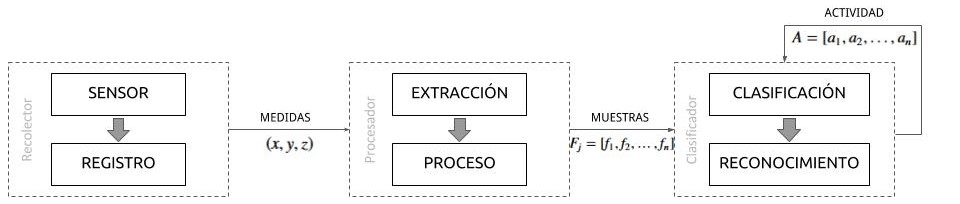
\includegraphics[width=1\linewidth]{capitulo-4/graphics/diagrama_4_1}\caption{Componentes de los sistemas HAR}
\label{fig41:componentes-har}
\end{figure}


\subsection{Recolector de datos}

El recolector de datos tiene la función de capturar medidas de los
sensores e registrar la información indexada en la dimensión del tiempo.
La captura de datos relevantes para los sistemas \abbr{HAR} debe
ser realizada con instrumentos de medición apropiados: en nuestro
caso con sensores (\abbr{Wearables}, o de atuendo). Los sensores
adjuntos se utilizan para recolectar señales directamente de los usuarios.
Estos están anexados a diferentes partes del cuerpo como la cintura,
la muñeca, el pectoral, los muslos o la cabeza \cite{Bao2004}, como
también ser portados ya que pueden estar empotrados en dispositivos
de uso regular como teléfonos móviles modernos, relojes inteligentes
o lentes \cite{LaraLabrador2012,Choudhury2008}.

\subsubsection{Sensores \emph{Wearables}}

Los sensores anexos directamente a un individuo pueden caracterizarse
según los siguientes atributos \cite{LaraLabrador2013}:
\begin{description}
\item [{Ubicación}] miden datos obtenidos con las redes celulares 3G y
los satélites de navegación \abbr{GPS}. Provee información de contexto
bastante relevante acerca de la posición del individuo, además de
ciertas medidas de movimiento pero con un consumo moderado de energía.
\item [{Movimiento}] miden datos inerciales como la aceleración y la orientación
respecto a un marco de referencia relativo al dispositivo que contiene
los sensores. El acelerómetro, giroscopio y la brújula son los sensores
más comunes y utilizados para reconocimiento de actividades con un
bajo consumo de energía y buena precisión de reconocimiento \cite{Bao2004,LaraLabrador2012}.
\item [{Fisiología}] miden signos vitales del individuo como el ritmo cardíaco
(\abbr{HRM}, \emph{Hearth Rate Monitor}), la temperatura del cuerpo,
el ritmo de respiración, entre otros.
\item [{Ambiental}] miden datos externos que rodean al individuo como el
nivel de ruido, la humedad y/o la temperatura. Los sensores de luz,
cámara, micrófonos y termómetros miden estos datos. 
\end{description}
Las señales medidas deben ser registrados de manera secuencial y transmitidos
para su posterior procesamiento. En ambas etapas, aprendizaje y predicción,
se miden las señales de los sensores.

\subsection{Procesador de muestras}

que procesa los datos en bruto para adecuarlos muestras con variables
significativas que permitan discriminar las actividades a reconocer

\subsection{Clasificador}

que utiliza las muestras extraídas para inferir qué actividad probable
está realizando un individuo en un determinado instante.

\section{Capacidades}

Existen un conjunto de características deseables que deben ser satisfechas
para la construcción efectiva de los sistemas de reconocimiento. Estas
características abordan cuestiones de diseño importantes que conciernen
a la calidad y al funcionamiento del sistema:
\begin{enumerate}
\item Portabilidad, el sistema utiliza sensores adjuntos a los individuos
(Ej. el acelerómetro) y no deben obstruir las actividades cotidianas
de los usuarios durante su uso. El fin es de evitar que se afecte
la adopción masiva del sistema. 
\item Conectividad, el sistema debe transmitir de manera confiable los datos
recolectados y/o procesados a algún componente desplegado de forma
remota. 
\item Almacenamiento, el sistema debe persistir los datos recolectados y/o
procesados de manera local en el dispositivo móvil con el fin de mantener
la calidad y minimizar la cantidad transferida a otros componentes.
\item Procesamiento, el sistema debe procesar y transformar los datos en
bruto para producir información relevante para el reconocimiento de
actividades.
\item Ubiquidad, el sistema debe operar en cualquier condición y contexto
en que la persona se encuentre sin interferir u obligar al usuario
a interactuar con el sistema.
\item Uso de energía, el sistema debe preservar el uso de energía en los
dispositivos móviles que están implementados. La lectura de datos,
el procesamiento y la conectividad no deben incurrir en gastos excesivos
de energía para que el sistema pueda operar.
\item Privacidad, el sistema debe mantener de manera confidencial los datos
recolectados y/o producidos durante la adopción masiva del sistema,
además de alertar sobre la utilización de datos sensibles que requieran
el consentimiento del usuario.
\end{enumerate}

